\chapter{INTRODUCTION}
%Chapter 1
%%%%%%%%%%%%%%%%%%%%%%%%%%%%%%%%%%%%%%%%%%%%%%%%%%%%%%%%%%%%%%%%%%%%%%%%%%%%%%%%%%%%%%%%%%%%%%%%%%%%%%%%%%%%%%%%%%%%%%
 In This thesis, we are presenting the study on two problems, $Steiner Tree$ and $All$-$pair$ $shortest$-$path$ problem, and with the help of 
 all-pairs shortest-path, we will reduce the running time of approximation algorithms for Steiner tree. Mainly we will focus on Steiner Tree problems. In this chapter, we present a brief introduction to both the problems. Also, some preliminaries and basic definitions that are used throughout this thesis. And what are the present approximation algorithms for the Steiner tree, which are fastest algorithms for constructing a minimum Steiner tree for a given graph $G$.
 
 \section{Overview and Motivation}
 \subsection{Steiner Tree Problem}
 $\emph{Steiner Tree Problem}$ $(\textsc{STP})$  Problem of Steiner tree is one of the combinatorial optimization problem, which is used in a number of applications, applications in an area like in which some items or points having some common property, we called these types of items or points as the required points in perspective of Steiner tree. So we are required to find the interconnections between these require points with minimum weight or cost of covering these points. While eliminating some unnecessary points, we can use these points, in the formation if these points, helping in construction of the minimum Steiner tree.

 $\textsc{STP}$ problem can be defined as follows:
 
 \begin{tabular}{|ll|}
 \hline
 \multicolumn{ 2}{|l|}{\problemfontbold{Steiner Tree Problem($\textsc{STP}$)}} \\
 \emph{INPUT} & \begin{minipage}[t]{0.75\columnwidth}
 Given a connected undirected graph $G$ = $(V,E)$ and weight of edges\\ $c$:$E$ $\rightarrow$ $\mathbb{R}_{\geq 0}$, a subset of nodes $S$ $\subseteq$ $V$, where $S$ is called as the required\\ vertices(Terminals) given as the input.
 \end{minipage} \\
 \emph{OUTPUT} & \begin{minipage}[t]{0.75\columnwidth}
 A Steiner Tree $T_s$, for Graph $G$ and $S$.
 \end{minipage}
 \\
 \hline
 \end{tabular}
 \\

 Finding the shortest path between two places is an important problem in real life applications and technology. The shortest path problem is also studying in the context of the communication networks. In communication networks, it is important to send data from one hub to other through a shortest available path. In the twentieth century, the development of communication networks forced researchers to design more efficient algorithms for better communication. Here we are presenting some motivational application of Steiner tree problem. Suppose, India want to start some new communication technology between some cities, Let technology is very useful for country, but installation may be costly, but have to start this technology, suppose Indian government is thinking of starting this technology in four major city like Delhi, Mumbai, Kolkata and Chennai, but starting this communication direct to direct from one city to other city it may be costly in some situation like direct linking between cities, there may be a chance of reducing the cost of communication and installation by using some other cities as the intermediary for providing connection between these four cities.

 This type of problem comes under the category of Steiner tree problem, as in Steiner tree problem we are given the required nodes and some non-required nodes, we have to find the connection between the required nodes with minimum cost of interconnection, in this connection we can use some of the non-required nodes. Same case in Steiner tree problem, in that we have to find a minimum cost tree connecting between all the required vertices, these required vertices called terminal vertices, these nodes are basically a subset of the nodes of the connected undirected, weighted graph $G$. Steiner tree problem is NP-Hard. Unless P=NP, there is no polynomial time algorithm for finding optimal solution for Steiner tree problems, so we cannot use well known currently available algorithms for finding an optimal solution of the problems. If we applied some constraints on these problems, then we may be a chance of solving some of the problems in polynomial time. So we have to think for solution in different way, our focus is to find a better algorithm for solving the problems, but there is no polynomial time algorithm for solving NP-Hard problems in polynomial time, so we have to change our approach for solving these problems, so now we are focusing on the better approximation algorithms with good running time.

  Till now best known approximation bound for Steiner tree problems is 1.55 given by Robins and Zelikovsky[2000]~\cite{hougardy}. There is no improvement for a long time in this Approximation, So we have to think problem differently to get the best approximation. For this our focus is on the LP-Based approximation like directing-component cut relaxation and Iterative randomized rounding. By LP-Based we are getting an approximation (ln 4 + $\in$) factor for some graph~\cite{byrka}.

  In this report our focus is to get the better run time for approximation algorithms. We will test the algorithm by running a test instance provided for the Steiner tree.\\


 \begin{tabular}{|ll|} 
 \hline
 \multicolumn{ 2}{|l|}{\problemfontbold{Steiner Tree Problems}} \\
 \emph{GOAL} & \begin{minipage}[t]{0.75\columnwidth}
 A MST that cover all the required vertices with minimum cost.
 \end{minipage} \\
 \emph{INPUT} & \begin{minipage}[t]{0.8\columnwidth}
 A connected undirected graph $G$ = $(V,E)$ with edge costs $c$:$E$ $\rightarrow$ $\mathbb{R}_{\geq 0}$,\\ and a subset of nodes $S$ $\subseteq$ $V$,  $S$ is called as the required nodes.
 \end{minipage} \\
 \emph{OUTPUT} & \begin{minipage}[t]{0.75\columnwidth}
 A Steiner Tree $T_s$, for Graph $G$ and $S$.
 \end{minipage}
 \\
 \hline
 \end{tabular}
 \\

 In figure 1.1, dark vertices are representing the required vertices, while hollow vertices representing the Steiner vertices, so we are required to cover every required vertices of the graph $G$ with the optimal cost, cost is the total sum of the edge weight that are participating in the Steiner tree formation. In figure 1.2, dark edges represent the Steiner tree that cover every terminal(require) vertices by using some of the Steiner vertices, the cost of covering all the require vertices is minimum, as there is no other tree that cover all the require vertices minimum cost which is less than that, and cover all the require vertices.

% \begin{figure}
%\begin{center}
\begin{figure}
\begin{center}
\centering
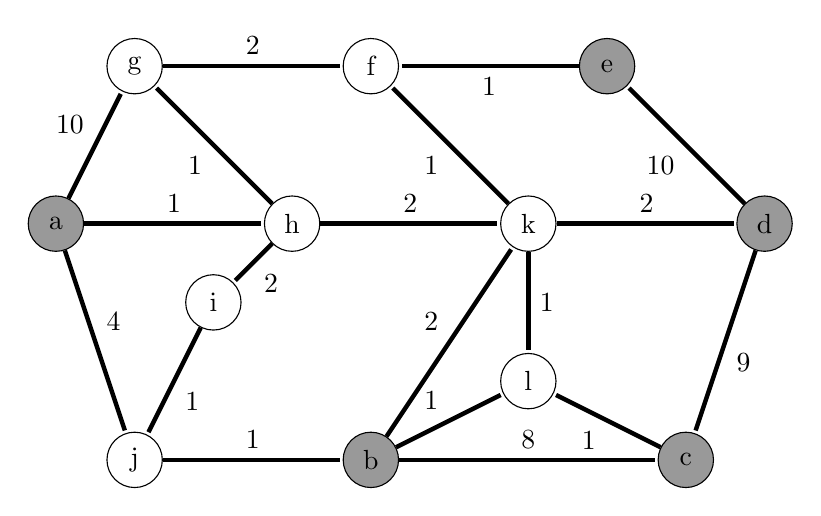
\begin{tikzpicture}[shorten >=1pt, auto, node distance=2cm,
   node_style/.style={circle,draw=black,minimum size = 20pt},
   edge_style/.style={draw=black, ultra thick}]

    \node[node_style] (v1) at (-1,0) {h};
    \node[node_style, fill=black!40] (v2) at (-4, 0) {a};
    \node[node_style] (v3) at (2,0)  {k};
    \node[node_style,fill=black!40] (v4) at (5,0)  {d};

    \node[node_style] (v5) at (-3,2) {g};
    \node[node_style] (v6) at (0,2)  {f};
    \node[node_style] (v7) at (-3,-3) {j};
    \node[node_style] (v8) at (-2,-1) {i};
    \node[node_style,fill=black!40] (v9) at (0,-3)  {b};
    \node[node_style] (v10) at (2,-2) {l};
    \node[node_style,fill=black!40] (v11) at (4,-3) {c};
    \node[node_style,fill=black!40] (v12) at (3,2)  {e};
    \draw[edge_style]  (v2) edge node{10} (v5);
    \draw[edge_style]  (v2) edge node{1} (v1);
    \draw[edge_style]  (v2) edge node{4} (v7);
    \draw[edge_style]  (v1) edge node{2} (v3);
    \draw[edge_style]  (v1) edge node{2} (v8);
    \draw[edge_style]  (v1) edge node{1} (v5);
    \draw[edge_style]  (v8) edge node{1} (v7);
    \draw[edge_style]  (v7) edge node{1} (v9);
    \draw[edge_style]  (v9) edge node{2} (v3);
    \draw[edge_style]  (v9) edge node{1} (v10);
    \draw[edge_style]  (v3) edge node{2} (v4);
    \draw[edge_style]  (v3) edge node{1} (v10);
    \draw[edge_style]  (v11) edge node{1} (v10);
    \draw[edge_style]  (v4) edge node{10} (v12);
    \draw[edge_style]  (v4) edge node{9} (v11);
    \draw[edge_style]  (v3) edge node{1} (v6);
    \draw[edge_style]  (v5) edge node{2} (v6);
    \draw[edge_style]  (v12) edge node{1} (v6);
    \draw[edge_style]  (v9) edge node{8} (v11);
    \end{tikzpicture}
    \caption{\small \sl A connected Graph $G$, with edges weights, having Steiner vertices(hallow) and terminal vertices(dark) \label{fig:sccEx} }
    \end{center}
    \end{figure}
\begin{figure}
\begin{center}
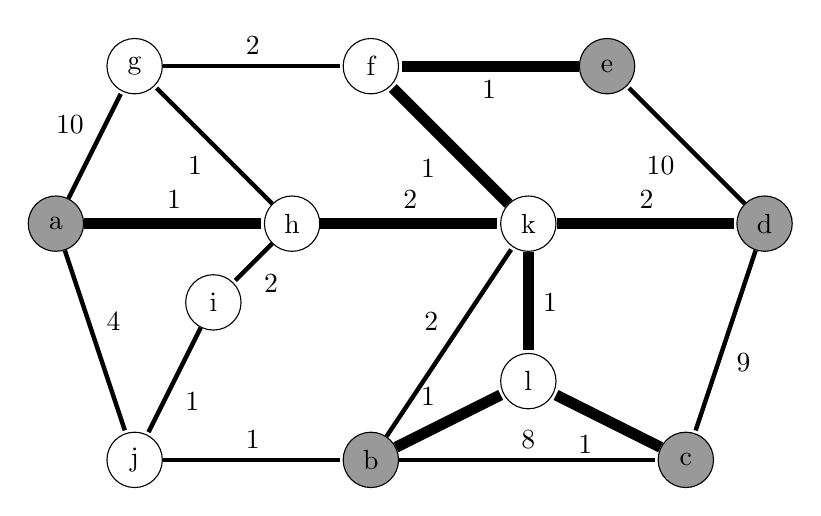
\begin{tikzpicture}[shorten >=1pt, auto, node distance=2cm, 
   node_style/.style={circle,draw=black,minimum size = 20pt},
   edge_style/.style={draw=black, ultra thick}]

    \node[node_style] (v1) at (-1,0) {h};
    \node[node_style, fill=black!40] (v2) at (-4, 0) {a};
    \node[node_style] (v3) at (2,0)  {k};
    \node[node_style,fill=black!40] (v4) at (5,0)  {d};

    \node[node_style] (v5) at (-3,2) {g};
    \node[node_style] (v6) at (0,2)  {f};
    \node[node_style] (v7) at (-3,-3) {j};
    \node[node_style] (v8) at (-2,-1) {i};
    \node[node_style,fill=black!40] (v9) at (0,-3)  {b};
    \node[node_style] (v10) at (2,-2) {l};
    \node[node_style,fill=black!40] (v11) at (4,-3) {c};
    \node[node_style,fill=black!40] (v12) at (3,2)  {e};
    \draw[edge_style]  (v2) edge node{10} (v5);
    \draw[edge_style, line width=4pt]  (v2) edge node{1} (v1);
    \draw[edge_style]  (v2) edge node{4} (v7);
    \draw[edge_style, line width=4pt]  (v1) edge node{2} (v3);
    \draw[edge_style]  (v1) edge node{2} (v8);
    \draw[edge_style]  (v1) edge node{1} (v5);
    \draw[edge_style]  (v8) edge node{1} (v7);
    \draw[edge_style]  (v7) edge node{1} (v9);
    \draw[edge_style]  (v9) edge node{2} (v3);
    \draw[edge_style, line width=4pt]  (v9) edge node{1} (v10);
    \draw[edge_style, line width=4pt]  (v3) edge node{2} (v4);
    \draw[edge_style, line width=4pt]  (v3) edge node{1} (v10);
    \draw[edge_style, line width=4pt]  (v11) edge node{1} (v10);
    \draw[edge_style]  (v4) edge node{10} (v12);
    \draw[edge_style]  (v4) edge node{9} (v11);
    \draw[edge_style, line width=4pt]  (v3) edge node{1} (v6);
    \draw[edge_style]  (v5) edge node{2} (v6);
    \draw[edge_style, line width=4pt]  (v12) edge node{1} (v6);
    \draw[edge_style]  (v9) edge node{8} (v11);
    \end{tikzpicture}
    % \caption{\small \sl Torricelli point X \label{fig:sccEx} }
    \end{center}
    \caption{\small \sl A Graph G, with edges weights and Steiner vertices as hollow vertices, terminal vertices(dark) and Steiner tree(dark edges) \label{fig:sccEx} }
    \end{figure}
\subsection{Terminal Steiner Tree}
 For a given graph $G$, Steiner tree whose all terminal vertices are of degree one, i.e., all the required vertices which are covered by the tree to form Steiner tree of minimum cost are leaves. All the require nodes of the Steiner tree must be leaves, but there is no restriction on the require nodes in the Steiner tree. In Steiner tree terminal node can also be some internal node. For example, in figure 1.3(a), a Steiner tree is formed from the a given graph $G$, in that Steiner tree some of the internal nodes are also terminal node. While in figure 1.3(b), a Steiner tree all the required vertices are leaves only, so this Steiner tree is called as the terminal Steiner tree.\\

 \begin{tabular}{|ll|} 
 \hline
 \multicolumn{ 2}{|l|}{\problemfontbold{Terminal Steiner Tree}} \\
 \emph{INPUT} & \begin{minipage}[t]{0.8\columnwidth}
  A connected weighted graph $G$ = $(V,E)$ with edge costs $c$:$E$ $\rightarrow$ $\mathbb{R}_{\geq 0}$, and\\ a subset of nodes $S$ $\subseteq$ $V$, $S$ is call required vertices (Terminals) as a input.
 \end{minipage} \\
 \emph{Output} & \begin{minipage}[t]{0.8\columnwidth}
 A Steiner tree $T_s$ of $G$, such that all the terminal node must be of degree one.
 \\	
 \end{minipage}
 \\
 \hline
 \end{tabular}
 
 \begin{figure}
\centering
\begin{subfigure}{.5\textwidth}
  \centering
    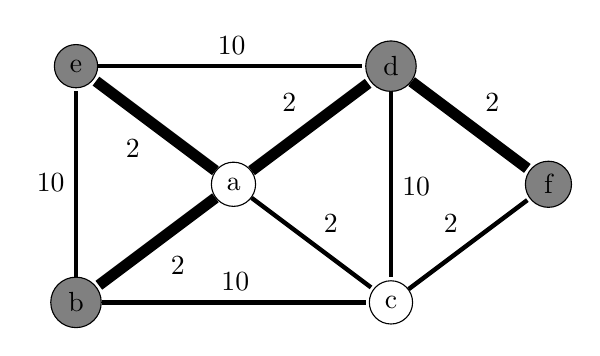
\begin{tikzpicture}[shorten >=1pt, auto, node distance=2cm,
            node_style/.style={circle,draw=black,minimum size = 10pt},
            edge_style/.style={draw=black, ultra thick}]
    \node[node_style] (v1) at (0,0.5)  {a};
    \node[node_style,fill=black!50] (v2) at (-2,-1) {b};
    \node[node_style] (v3) at (2,-1)  {c};
    \node[node_style,fill=black!50] (v4) at (2,2) {d};
    \node[node_style,fill=black!50] (v5) at (-2,2) {e};
    \node[node_style,fill=black!50] (v6) at (4,0.5) {f};

    \draw[edge_style, line width=4pt]  (v1) edge node{2} (v2);
    \draw[edge_style]  (v1) edge node{2} (v3);
    \draw[edge_style, line width=4pt]  (v1) edge node{2} (v4);
    \draw[edge_style, line width=4pt]  (v1) edge node{2} (v5);
    \draw[edge_style]  (v2) edge node{10} (v5);
    \draw[edge_style]  (v2) edge node{10} (v3);
    \draw[edge_style]  (v5) edge node{10} (v4);
    \draw[edge_style]  (v4) edge node{10} (v3);
    \draw[edge_style, line width=4pt]  (v4) edge node{2} (v6);
    \draw[edge_style]  (v3) edge node{2} (v6);
    \end{tikzpicture}
  
  % \includegraphics[width=.4\linewidth]{image1}
  \caption{Steiner tree of a graph with four terminals}
  \label{fig:sub1}
\end{subfigure}%
\begin{subfigure}{.5\textwidth}
  \centering
  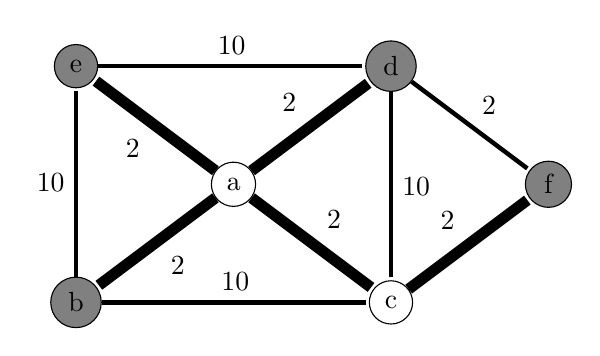
\begin{tikzpicture}[shorten >=1pt, auto, node distance=2cm,
            node_style/.style={circle,draw=black,minimum size = 10pt},
            edge_style/.style={draw=black, ultra thick}]
    \node[node_style] (v1) at (0,0.5)  {a};
    \node[node_style,fill=black!50] (v2) at (-2,-1) {b};
    \node[node_style] (v3) at (2,-1)  {c};
    \node[node_style,fill=black!50] (v4) at (2,2) {d};
    \node[node_style,fill=black!50] (v5) at (-2,2) {e};
    \node[node_style,fill=black!50] (v6) at (4,0.5) {f};

    \draw[edge_style, line width=4pt]  (v1) edge node{2} (v2);
    \draw[edge_style, line width=4pt]  (v1) edge node{2} (v3);
    \draw[edge_style, line width=4pt]  (v1) edge node{2} (v4);
    \draw[edge_style, line width=4pt]  (v1) edge node{2} (v5);
    \draw[edge_style]  (v2) edge node{10} (v5);
    \draw[edge_style]  (v2) edge node{10} (v3);
    \draw[edge_style]  (v5) edge node{10} (v4);
    \draw[edge_style]  (v4) edge node{10} (v3);
    \draw[edge_style]  (v4) edge node{2} (v6);
    \draw[edge_style, line width=4pt]  (v3) edge node{2} (v6);
    \end{tikzpicture}
  
  % \includegraphics[width=.4\linewidth]{image1}
  \caption{Terminal Steiner tree of a Graph G}
  \label{fig:sub2}
\end{subfigure}
\caption{Terminal Steiner Tree in which all the degree vertices are terminals, while in case of Steiner tree some internal node can also be terminal nodes.}
\label{fig:test}
\end{figure}
\section{Applications of Steiner Tree}
 The Steiner tree problems have so many applications like in circuit layout, network design, and telephone communications. Everywhere where the shortest path required between the interconnecting, some of the require points with some specific properties and we are required to connect these points with the help of some optional points, there we can use Steiner tree.
  Here are the some applications of Steiner tree.\\
 \textbf{In physical VLSI designs:-}
  Steiner tree is used, whenever the placement of component on a chip, there may be a chance that, a set of pin are to be connected with in the free space. A set pin which sharing the networks in the designs, these pins are called as the required vertices, and some other pins which are not useful in the network designs, but with the help of these pins we may connect the require vertices in designing of the network. with the help of these optional pins, we may connect the required pins and fulfil the purpose of the require pins in the designs of networks.\\
 \textbf{On-line and Dynamic Steiner tree:-}
 On-line application of the Steiner tree comes, whenever a new change in the network because of some new additional points for service, then there is a requirement of new connection in the telephone network. If a new points for the service is added then, a new line of connect for the new point in the network has to build. In this network construction is like a way the every time, whenever location is change a new network is formed based on the previous network. this brings us a issue of dynamic Steiner tree, in that whenever new network is built, we have to calculate an approximation for the performance of the network.
 \section{Existing Approximation Algorithms}
 There are series of research in the improvement the approximation ratio of the Steiner tree problems. It starts from 2-approximation and after so many of the  improvement it reached to 1.55, i.e., the best known approximation by Robins and Zelikovsky[2000] ~\cite{hougardy}.\\\
Here is the list of Existing approximation ratio for the Steiner tree ~\cite{hougardy}.\\
\begin{table}[h]
% \caption{My caption}
\label{my-label}
\begin{center}
\begin{tabular}{|l|l|l|l|l|l|l|l|l|}
\hline
Approximation Bound & References \\ \hline
    2.0-approximation  & minimum spanning tree heuristic \\ \hline
    1.83-approximation & Zelikovsky 1993   \\ \hline
    1.78-approximation & Berman and Ramaiyer 1994 \\ \hline
    1.73-approximation & Borchers and Du 1997 \\ \hline
    1.67-approximation & Pr\"{o}mel and Steger 1997 \\ \hline
    1.65-approximation & Karpinski and Zelikovsky 1997 \\ \hline
    1.59-approximation & Hougardy and Pro\"{o}mel 1999 \\ \hline
    1.55-approximation & Robins and Zelikovsky 2000 \\ \hline

         % &        &        &        &           &        &        &       &          \\ \hline
         % &        &        &        &           &        &        &       &          \\ \hline
\end{tabular}
\end{center}
\caption{Existing approximation ratio for the Steiner tree}
\end{table}
A series of improvement, maximize with Robins and Zelikovsky's ~\cite{byrka} famous 1+$\frac{ln(3)}{2}$ + $\epsilon$ $<$ 1.55 (here $\epsilon$ $>$0 is an arbitrary small constant) algorithm improved this ratio by iteratively improving upon the minimum weight terminal Steiner tree. The above results are based on the Steiner tree as a full components. A component of the Steiner tree is the tree whose all the required(terminal) vertices are the leaves of the tree. But considering the full component at a time will not give a good approximation ratio. If we consider the Steiner tree with special structure, So called r-restricted Steiner, in this tree every components that have no more than r-terminals. To get a better approximation, It is better to pay attention to r-restricted Steiner tree. By using this approach we may get a better approximation ratio ~\cite{byrka}.\\
{\textbf{Steiner Ratio:-} The Ratio between the total length of the minimum Steiner tree and the total length of a minimum Spanning tree, Steiner ratio represented as $\rho$.
\section{All-Pairs Shortest-Paths Algorithm}

 All-Pair Shortest-path(APSP) problem is one of the fundamental problems in the graph theory. A classical ways for solving 
 $\textsc{APSP}$ in general weighted graphs is given by Floyd and Warshall ~\cite{cormen}. It outputs an $V$ $\times$ $V$ matrix, in that every pairs of vertices at the minimum distance, it takes $\Theta(V^3)$ time. In all-pairs Shortest-paths problem, 
 we are required to find the shortest path between each and every pairs of vertices of the graph $G$ = $(V,E)$. $i.e.,$ we are given a $V_i$ and $V_j$ where $(V_i,V_j)$ $\in$ $V$, this algorithm used to find the shortest paths between vertices $V_i$,$V_j$. All-Pairs Shortest-Paths problem can be solved by using the a single-source shortest-path algorithm by running $|V|$ times to find the shortest path for each and every vertex of the graph as a source. With the help of All-Pairs Shortest-paths
 algorithms, we are coming up a better running time approximation algorithm for Steiner tree, this algorithm will be better only for those graph which have edges of order $O(E)$ $\leq$ $|V|log|V|$. Running time of an algorithm totally depends 
 on algorithmic and data-structure that we are using in the implementation.   

\section{Preliminaries}

\textbf{Weighted Graph:-} A graph has two elements, vertices and edges. The edges connecting the two end points or vertices of the graph, have some cost of connecting two vertices, this is called as the weight for that edge. If weights are associated with every edge, this type of graph called as the weighted graph. Weight sum of all the edges is called as the weight of graph. \\ 
 \textbf{Path in a Graph:-} A path is a sequence of edges which connects the vertices of the graph. The Sum of all associated weights with edges so called as the weight of the path.\\
 \textbf{Subgraph:-} A subgraph $P$ is the subgraph of the graph $G$, whose edges and vertices are the subset of the $G$.\\
 \textbf{Tree:-} A tree is a acyclic graph. A tree is a graph is which every vertex is connected with exactly one path, one degree vertices are called as the leaves of the tree. Tree became disconnected after removal of any edges.\\
 % \textbf{Degree of the vertices:-} Number of edges connected to a vertex is known as the degree of that vertex.\\
 \textbf{Minimum Spanning Tree:-} A spanning tree of a graph is the tree which connects every vertices of the graph, A minimum spanning tree is the tree which have optimal cost of covering every vertices. i.e., there is no other tree having weight less than a minimum spanning tree. The sum of all the weight of all the edges of tree is called as the weight of the minimum spanning tree. Algorithms for finding the minimum spanning tree in a graph are Prim's algorithm, kruskal's algorithm.\\
 \textbf{Dijkstra's Algorithm:-} Dijkstra's algorithm one of the shortest path algorithm, it use single vertex as a source for finding the shortest path. Run time complexity of this algorithm is $O(|E| + |V|log|V|)$, if we use fibonacci heap as in implementation, where $|E|$ is the number of edges.\\
 \textbf{Sparse Graph:-} A graph in which number of edges are much less than the possible number of edges.
 \section{Contribution of the Thesis}
 In this thesis, we restrict our attention on fastest approximation algorithm for Steiner tree. Not only on the theoretical interest about the approximation algorithm of the Steiner tree, But also on the practical impact of the algorithms are present in this thesis.
 All-Pairs Shortest-Paths algorithms have been shown to find some better solution in practice for approximation algorithm, But because of the high run time on a big graph and different type of problems limits their applicability. Underlying graph structure can play an important role in setting up efficient approximation algorithms. All-pairs shortest-paths algorithms, tries to improve an existing solution by modifying the current exiting algorithm, for finding the best path between the pair of terminals. In this All-pairs shortest paths basically focusing on the find the best minimum path between the terminals, by that it for providing some better  solution for our approximation algorithm, if we apply some change in algorithm. By this way we may get better run time for some limited problems, This is also confirming that non-trivial data-structures and algorithmic are also very important for the solution of some real-world problems for optimization. 
 \section{Organization of the Thesis}
 This thesis is organized in 5 chapters. Current chapter is an introduction to the thesis. It contains an introduction           
 and motivation for the Steiner tree problem. We presented some graph theoretic preliminaries which are used throughout this thesis.
 In Chapter \ref{ch_prelim} we study various types of Steiner tree and existing algorithms, and we explained some of the approximation algorithms. Also, we prove the various important properties of Steiner tree. Chapter \ref{ch_review} presents a nice survey of the work done on all-pairs shortest-path algorithms and how, it will use in the Steiner tree algorithm for improving the running time for heuristic algorithm.
In chapter \ref{ch_distOracle} we present an algorithm to construct a shortest distance between all-pairs of terminals using APSP. How we are using this algorithm to solve the approximation algorithm for Steiner tree. Finally, Chapter \ref{ch_concl} concludes the thesis. This chapter also lists some interesting direction for research and open problems for further study, and some case that can be consider for further improvement in the approximation algorithms.